\myChapter{Results on parameter adaptation in heterogeneous machines}\label{chap:adaptiveresults}
\minitoc\mtcskip
\vfill
\lettrine{I}{n} this chapter OSGiLiath is used to execute the algorithms presented in Chapter \ref{chap:adaptive}. The implementation of the distributed islands is performed following the steps of the subsection \ref{subsec:migrator} of the Chapter \ref{chap:osgiliath}.

The three main objectives of parallel programming are to tackle large computational problems, increase the performance of algorithms in a finite time, or reduce computational time to solve the problem (reaching the optimum). In this chapter, we focus in the last objective.
As claimed by \person{Alba and Luque} in \cite{Alba06evaluationParallel}, assessing the performance of a parallel EA by the number of fitness function evaluations required to attain a solution may be misleading. In our case, for example, the evaluation time is different in each node of the heterogeneous cluster, so the real algorithm speed could not be reflected correctly. However, the number of evaluations has been included in this chapter to better understand the results. The total number of generations carried out by all nodes, and the maximum number of generations required by the faster node in each configuration are also shown. It is difficult to compare the performance of HoHa and HeHa for the same reason: the evaluation time is different in each system (and even in each node). Thus, one of the objectives in this thesis is not making the heterogeneous cluster comparable or better in time than the homogeneous one (because they are, obviously, different), but showing that the same parameter configuration can improve performance in time on heterogeneous clusters and could not have an effect on homogeneous ones.


\section{MMDP results}

Table \ref{tab:resultsMMDP} shows the results for the MMDP problem. These results are also shown in the boxplots of Figure \ref{fig:timeMMDP} (time) and Figure \ref{fig:evalsMMDP} (evaluations). Table \ref{tab:significanceMMDP} shows the statistical significance of the results. First, a Kolmogorov-Smirnov test is performed to assess the normality of the distributions. As all distributions are not normal, we use non-parametric tests. To compare between two methods (HoSi and HeSi in the homogeneous cluster) a Wilcoxon test has been applied. For a three methods comparison (HoSi, HeSi and AdSi on heterogeneous cluster) a Kruskal-Wallis test has been used. 

 In the HeHa system, adapting offline the sub-population to the computational
 power of each node makes the algorithm finish significantly earlier,
 and also, needing a lower number of evaluations to reach the solution. On the other hand, in the HoHa system,
 setting the same sub-population sizes makes no difference in time and
 evaluations, that is, changing this parameter has no influence in the
 algorithm's performance (p-value=0.52 for time and 0.08 for evaluations).


\begin{SCtable}[][t]
\resizebox{11cm}{!}{
\begin{tabular}{ccccc}
\hline
\rowcolor{colorCorporativoSuave}Configuration & Max. generations      & Total generations     &   Total evaluations     & Time (ms) \\ \hline \hline
\rowcolor{colorCorporativoMasSuave}HoSi/HeHa & 11194.8 $\pm$ 18810.08   & 30161.42 $\pm$  50722.03 & 7723372.8 $\pm$  12984841.71   & 27871.075 $\pm$  44583.14 \\ \hline
\rowcolor{colorCorporativoSuave}HeSi/HeHa   & 2506.1  $\pm$5308.872    & 8683.9    $\pm$ 18459.58 &  2453677 $\pm$5217896.18  &  8110.9 $\pm$ 17162.86 \\ \hline
\rowcolor{colorCorporativoMasSuave}AdSi/HeHa   & 2407.10 $\pm$3938.43     & 8376.35 $\pm$ 14140.55   & 2948946.15  $\pm$  5165324.99 &  10235.89  $\pm$ 17193.98\\ \hline  \hline
\rowcolor{colorCorporativoSuave}HoSi/HoHa   & 2614    $\pm$5889.93     & 10259.22  $\pm$ 23153.23 &  2628409.6 $\pm$   5927278.22 & 11560.8 $\pm$ 26072.14 \\ \hline
\rowcolor{colorCorporativoMasSuave}HeSi/HoHa   & 5411.92 $\pm$15608.81    & 10689.15  $\pm$  30790.7 & 1844908.1 $\pm$  5314771.88 &  9520.325 $\pm$   27237.35 \\ \hline

\end{tabular}
}
\caption{Results for the MMDP problem}
\label{tab:resultsMMDP}
\end{SCtable}




\begin{SCfigure}[htb]
\centering

%\subfigure[Heterogeneous cluster]{
   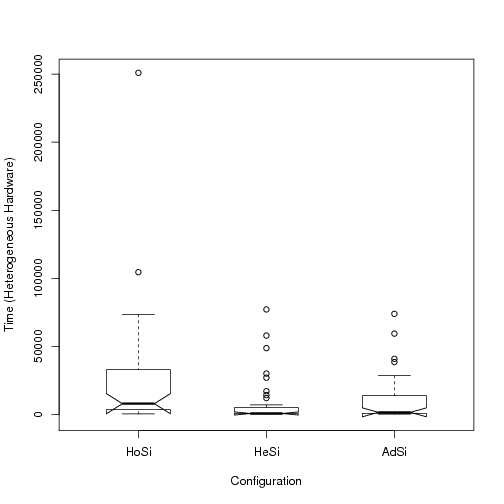
\includegraphics[scale =0.4] {gfx/adaptiveresults/timeMMDPhetero.png}
   \label{fig:subfig1}
%}
%\subfigure[Homogeneous cluster]{
   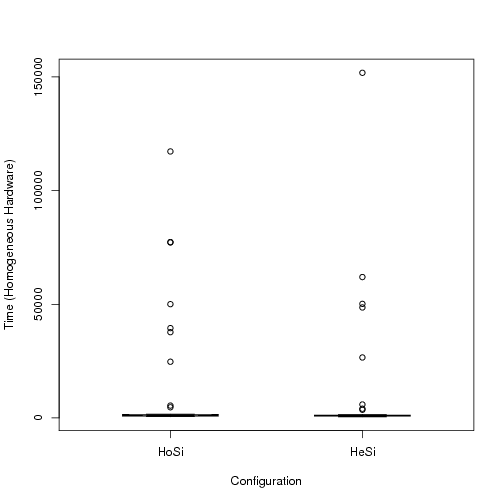
\includegraphics[scale =0.4] {gfx/adaptiveresults/timeMMDPhomo.png}
   \label{fig:subfig2}
% }
\caption{Time to obtain the optimum in the MMDP problem
  (milliseconds).}

\label{fig:timeMMDP}
\end{SCfigure}

\begin{SCfigure}[htb]
\centering

%\subfigure[Heterogeneous cluster]{
   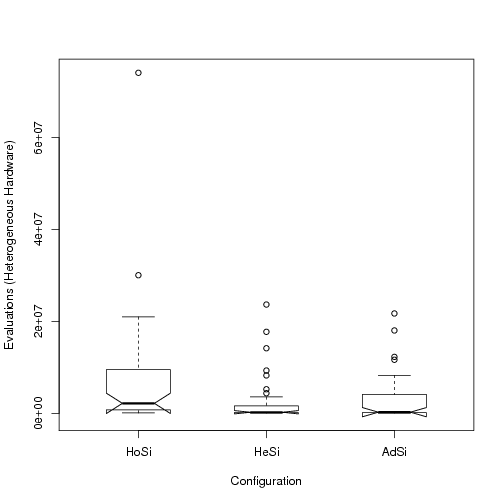
\includegraphics[scale =0.4] {gfx/adaptiveresults/evalsMMDPhetero.png}
   \label{fig:subfig1}
 %}
%\subfigure[Homogeneous cluster]{
   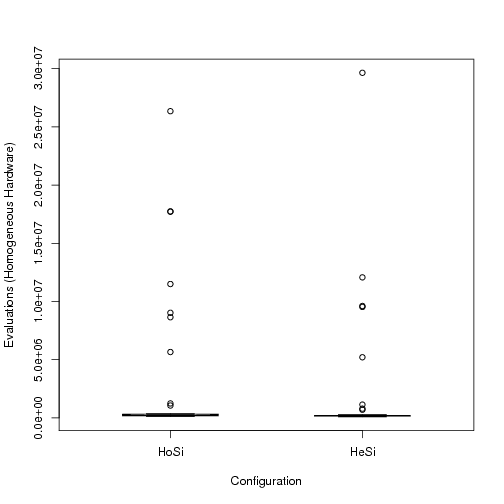
\includegraphics[scale =0.4] {gfx/adaptiveresults/evalsMMDPhomo.png}
   \label{fig:subfig2}
 %}
\caption{Number of evaluations for MMDP problem.}
\label{fig:evalsMMDP}
\end{SCfigure}



To see the differences on how the evolution is being performed, the average fitness in each node of HeHa is shown in Figures \ref{fig:hosiheha} and \ref{fig:hesiheha}. As it can be seen, with the HeSi (Figure \ref{fig:hesiheha}), the local optima are overtaken in less time than HoSi (Figure \ref{fig:hosiheha}).  This can be explained because in HeSi, the migration from HeN4 to HeN1 is performed faster, adding more heterogeneity to the whole system. Gaps in the figures correspond to the time spent in the nodes for sending the migrant individual to other nodes (not while they are receiving them). In the HoHa configurations, the evolution of sub-population is performed at the same time, being the average fitness similar in all nodes during all run. 


\begin{SCfigure}[htb]
\centering
 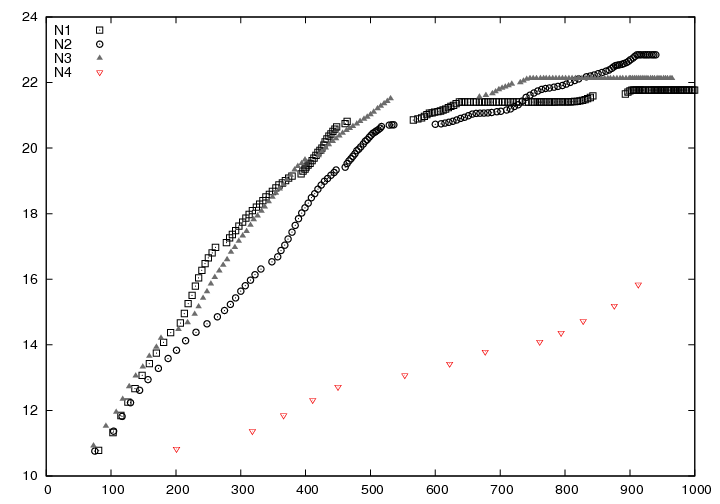
\includegraphics[scale =0.4] {gfx/adaptiveresults/generationsMMDPhomosize.png}
\caption{Average fitness in the first 1000 milliseconds of execution of the four nodes of the heterogeneous cluster with the same sub-population sizes (HoSi/HeHa) for the MMDP problem.}
\label{fig:hosiheha}
\end{SCfigure}

\begin{SCfigure}[htb]
\centering
 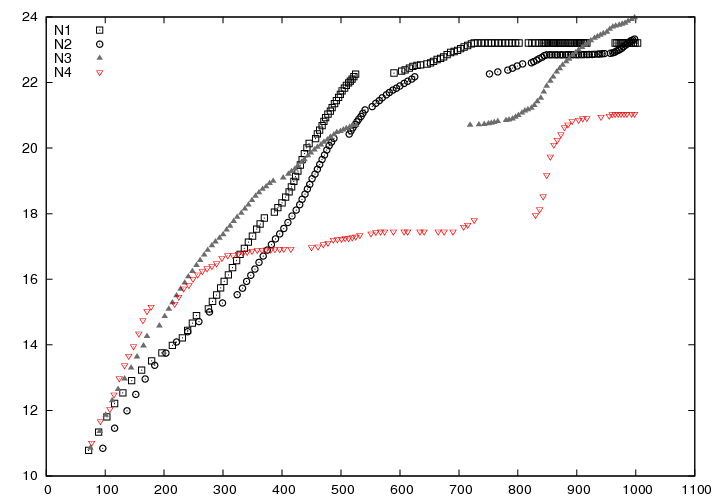
\includegraphics[scale =0.4] {gfx/adaptiveresults/generationsMMDPheterosize.png}
\caption{Average fitness in the first 1000 milliseconds of execution of the four nodes of the heterogeneous cluster with different sub-population sizes (HeSi/HeHa) for the MMDP problem.}
\label{fig:hesiheha}
\end{SCfigure}

Regarding to AdSi/HeHa, results are significantly  equal (p-value 0.139) to HeSi/HeHa (and, therefore, better than HoSi/HeHa), but this time no previous tuning has been required.  Average sub-population sizes in each node are shown in Table \ref{table:sizesMMDP}. The proportions of size are similar to the proportions in Table \ref{table:generations}. Figure \ref{fig:sizesMMDP} plots all the possible sizes in each node during all the runs. This figure shows that the variation of the sub-population sizes lies proportionally to the computational power of each node. The outliers in boxplots are produced during the size changing, as it can be seen in Figure \ref{fig:sizesMMDP1ejec}. As N4 is the slower node with difference it keeps its size always close to the minimum (16 individuals).

\begin{SCfigure}[htb]
\centering
 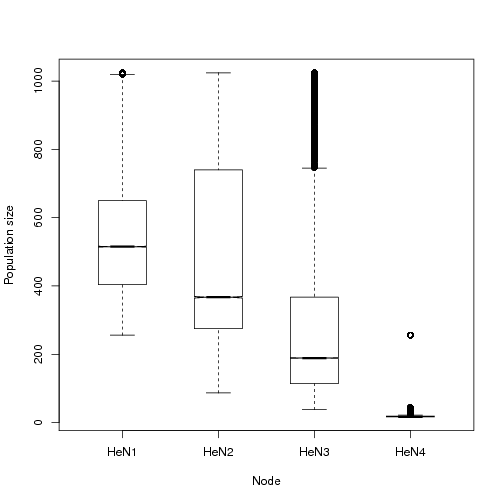
\includegraphics[scale =0.4] {gfx/adaptiveresults/sizesMMDP.png}
\caption{Boxplots of the sub-population sizes in each node during all the runs for the MMDP problem.}
\label{fig:sizesMMDP}
\end{SCfigure}

\begin{SCfigure}[htb]
\centering
 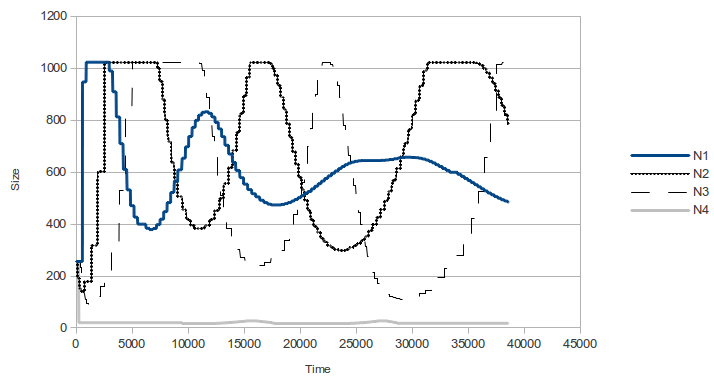
\includegraphics[scale =0.4] {gfx/adaptiveresults/sizesMMDP1ejec.png}
\caption{Population size in each node during one execution to solve the MMDP problem.}
\label{fig:sizesMMDP1ejec}
\end{SCfigure}



\begin{SCtable}[][htb]
\resizebox{6cm}{!}{
\begin{tabular}{ccccc}
\hline
\rowcolor{colorCorporativoSuave}Node        & HeN1     & HeN2      & HeN3     & HeN4   \\ \hline \hline
\rowcolor{colorCorporativoMasSuave}Size &  556.31 & 504.30  & 321.15 & 19.81 \\ \hline
\rowcolor{colorCorporativoSuave}Proportion  & 39.69 &  35.98 & 22.91 & 1.41   \\ \hline
\end{tabular}
\caption{Average sub-population size in each node on the heterogeneous cluster with adaptive size (MMDP).}
\label{table:sizesMMDP}
}
\end{SCtable}



Summarizing, adapting the sub-population sizes to the computational power of each machine (offline and online) has reduced the time to obtain the optimum. The same heterogeneous fixed sizes in the homogeneous cluster does not produces a significant decrease of running time, so the improvement is produced by the heterogeneity and not due to the different island sizes. Moreover, the AdSi proposal is not applicable in HoHa because there are not differences of generations during runtime.

\section{OneMax results}

Results for this problem are shown in Table \ref{tab:onemaxresults} and Figures  \ref{fig:timeOneMax} and \ref{fig:evalsOneMax}. In this case, adapting offline the sub-population sizes significantly decreases  the running time for solving it in the heterogeneous cluster, but this time, the number of evaluations is increased (see statistical significance in Table \ref{tab:significanceONEMAX}). In the homogeneous system, the effect of changing the sub-population sizes is clearer, and this time the number of evaluations (and therefore, the time) are reduced (both significantly). 

The efficiency on OneMax problem depends mainly on the ability to mix
the building-blocks, and less on the genetic diversity and size of the
population (as with MMDP). No genetic diversity is particularly
required. When properly tuned, a simple Genetic Algorithm is able to
solve OneMax in linear time. Sometimes, problems like OneMax are used
as control functions, in order to check if very efficient algorithms
on hard functions fail on easier ones. As it can be seen in Figure
\ref{fig:gensonemaxhomosize}, the average fitness of all sub-populations
are increasing in linear way in the HoSi/HeHa configuration. However,
the slower node evaluates extremely fewer times.  On the other

side, in Figure \ref{fig:gensonemaxheterosize}, smaller sub-population
sizes make that slower nodes increase the number of evaluations,
but the average fitness is also maintained in linear way (and in
smaller increase rate) between migrations. Nevertheless, the other
nodes still perform a higher number of evaluations. That is the
reason why the number of evaluations is higher in HeHa, and lower in
HoHa. Computational time is more efficiently spent in faster nodes,
having a higher chance to cross the individuals. In addition, due to
the larger size of  individuals in the OneMax problem (5000 bits
vs. 150 of the MMDP), the transmission time is larger, (white gaps in the
figures). It also implies that HeN4 sends its best individual to
HeN1 in an extremely large amount of time when using HoSi (every 64
generations). 


\begin{SCtable}[][htb]
\resizebox{11cm}{!}{
\begin{tabular}{ccccc}
\hline
\rowcolor{colorCorporativoSuave}Configuration & Max. generations      & Total generations     &   Total evaluations     & Time (ms) \\ \hline \hline
\rowcolor{colorCorporativoMasSuave}HoSi/HeHa   & 2430.34 $\pm$ 70.16  & 6299.31 $\pm$ 250.87 & 1614673.45  $\pm$  64223.09  &  160713.65 $\pm$   8873.46 \\ \hline
\rowcolor{colorCorporativoSuave}HeSi/HeHa   & 2643.34 $\pm$150.82  & 7969.58 $\pm$214.92 & 1802321.65  $\pm$  30511.96  &  151822.75  $\pm$4764.95 \\ \hline 
\rowcolor{colorCorporativoMasSuave}AdSi/HeHa   & 3698.30 $\pm$ 494.56 & 9465.25 $\pm$ 635.07 & 1149277.43  $\pm$ 58887.13 &  103919.33  $\pm$ 6296.39 \\ \hline \hline
\rowcolor{colorCorporativoSuave}HoSi/HoHa   & 1791.32 $\pm$   31.64& 7111.05 $\pm$125.11 & 1822476.8   $\pm$32029.78  &  141176.1    $\pm$2493.72\\ \hline
\rowcolor{colorCorporativoMasSuave}HeSi/HoHa   & 13698.12 $\pm$ 406.85 & 16012.625 $\pm$  482.61 & 895698.2 $\pm$   29520.99  &  77898.85  $\pm$  2935.57 \\ \hline
\end{tabular}
}
\caption{Results for the OneMax problem.}
\label{tab:onemaxresults}
\end{SCtable}



\begin{SCfigure}[htb]
\centering

%\subfigure[Heterogeneous cluster]{
    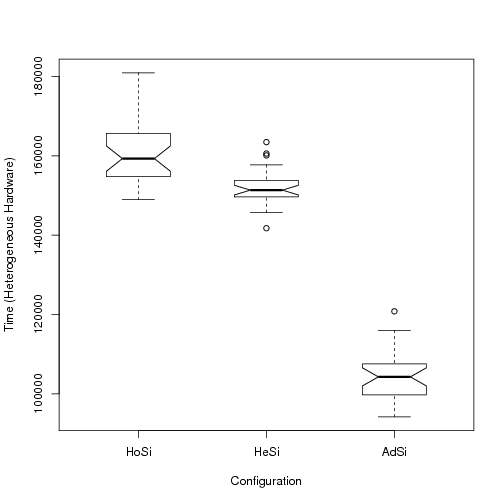
\includegraphics[scale =0.4] {gfx/adaptiveresults/timeONEMAXhetero.png}
   \label{fig:subfig1}
 %}
%\subfigure[Homogeneous cluster]{
    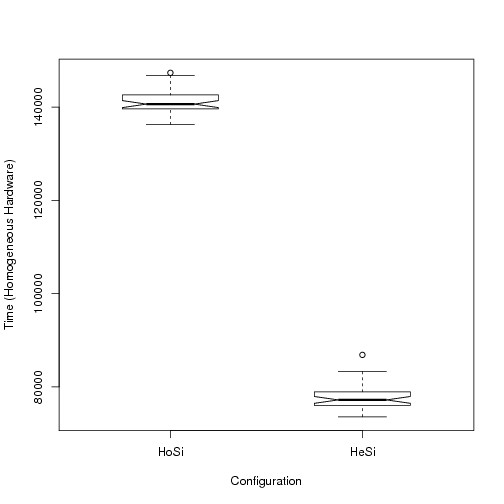
\includegraphics[scale =0.4] {gfx/adaptiveresults/timeONEMAXhomo.png}
   \label{fig:subfig2}
 %}
\caption{Time to obtain the optimum in the OneMax problem (milliseconds).}
\label{fig:timeOneMax}
\end{SCfigure}

\begin{SCfigure}[htb]
\centering

%\subfigure[Heterogeneous cluster]{
   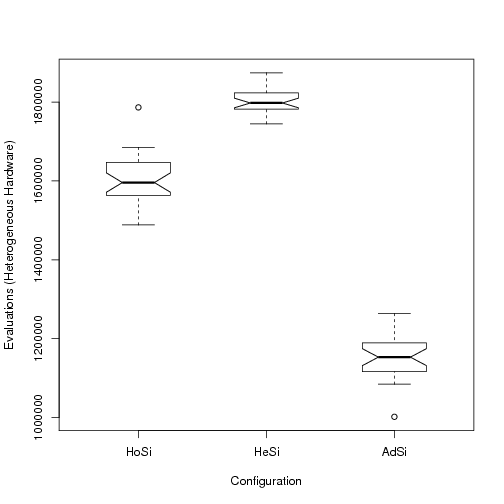
\includegraphics[scale =0.4] {gfx/adaptiveresults/evalsONEMAXhetero.png}
   \label{fig:subfig1}
 %}
%\subfigure[Homogeneous cluster]{
   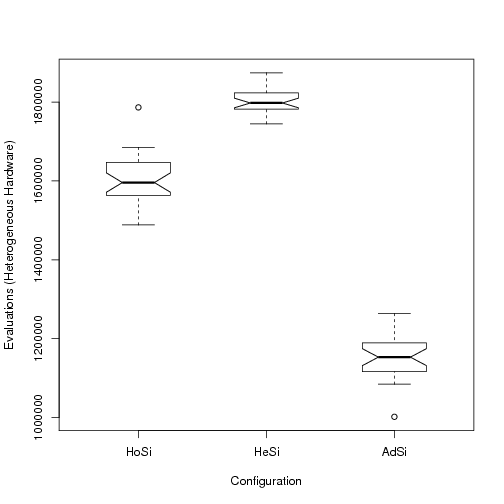
\includegraphics[scale =0.4] {gfx/adaptiveresults/evalsONEMAXhetero.png}
   \label{fig:subfig2}
 %}
\caption{Number of evaluations for OneMax problem.}
\label{fig:evalsOneMax}
\end{SCfigure}



\begin{SCfigure}[htb]
\centering 
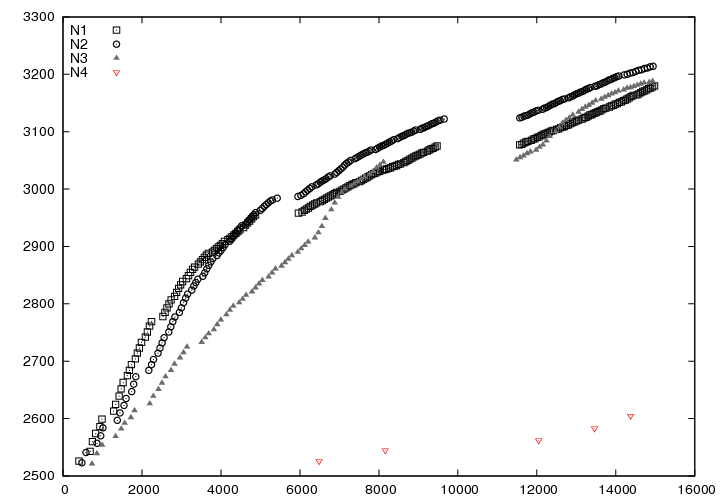
\includegraphics[scale =0.4] {gfx/adaptiveresults/generationsONEMAXhomosize.png}
\caption{Average fitness in the first 15000 milliseconds of execution of the four nodes of the heterogeneous cluster with the same sub-population sizes (HoSi/HeHa) for the OneMax problem.}
\label{fig:gensonemaxhomosize}
\end{SCfigure}

\begin{SCfigure}[htb]
\centering
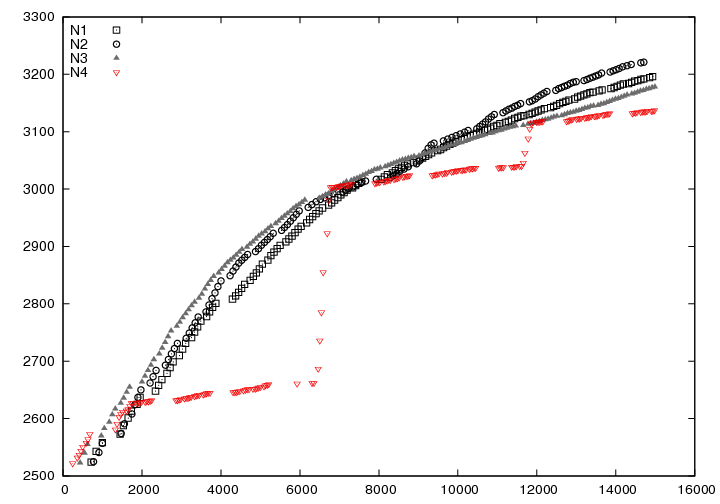
\includegraphics[scale =0.4] {gfx/adaptiveresults/generationsONEMAXheterosize.png}
\caption{Average fitness in the first 15000 milliseconds of execution of the four nodes of the heterogeneous cluster with different sub-population sizes (HeSi/HeHa) for the OneMax problem.}
\label{fig:gensonemaxheterosize}
\end{SCfigure}


In the AdSi/HeHa configuration significantly better results in terms of execution time (and number of evaluations) are also attained, and even better than those obtained with HeSi. Average sizes (Table \ref{table:sizesONEMAX}) and boxplots (in Figure \ref{fig:sizesONEMAX}) during all the runs also show proportionality to the computational power of each machine. As in MMDP case, some oscillations (outliers in boxplots) may appear during the execution (as it can be seen in Figure \ref{fig:sizesONEMAX1ejec}).

\begin{SCfigure}[htb]
\centering
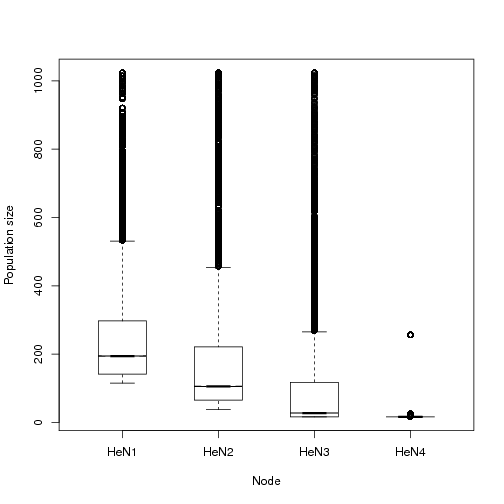
\includegraphics[scale =0.4] {gfx/adaptiveresults/sizesONEMAX.png}
\caption{Boxplots of the sub-population sizes in each node during all the runs for the OneMax problem.}
\label{fig:sizesONEMAX}
\end{SCfigure}

\begin{SCfigure}[htb]
\centering
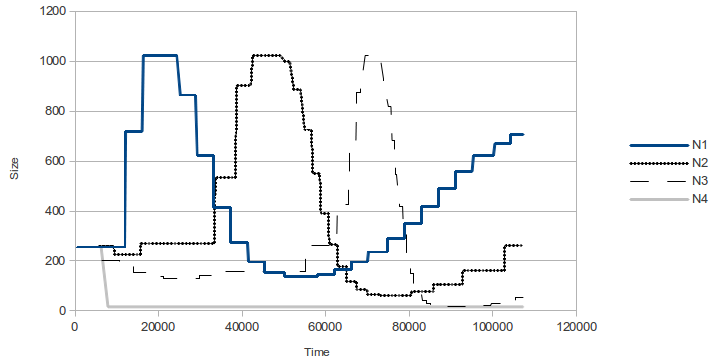
\includegraphics[scale =0.4] {gfx/adaptiveresults/sizesONEMAX1ejec.png}
\caption{Sub-population size in each node during one execution to solve the OneMax problem.}
\label{fig:sizesONEMAX1ejec}
\end{SCfigure}


\begin{SCtable}[][htb]
\resizebox{6cm}{!}{
\begin{tabular}{ccccc}
\hline
\rowcolor{colorCorporativoSuave}Node        & HeN1     & HeN2      & HeN3     & HeN4   \\ \hline \hline
\rowcolor{colorCorporativoMasSuave}Size &   267.09 & 158.63 &  74.20  & 16.29 \\ \hline
\rowcolor{colorCorporativoSuave}Proportion  &  51.73 &  30.72 &   14.37 &  3.15  \\ \hline
\end{tabular}
\caption{Average sub-population size in each node on the heterogeneous cluster with adaptive size (OneMax).}
\label{table:sizesONEMAX}
}
\end{SCtable}



\begin{SCtable}[][htb]
\resizebox{11cm}{!}{
\begin{tabular}{cccccc}
\hline

\multicolumn{6}{>{\columncolor{colorCorporativoSuave}}c}{Time} \\ \hline \hline
\multicolumn{6}{>{\columncolor{colorCorporativoMasSuave}}c}{Kruskal-Wallis chi-squared = 20.3042, df = 2, p-value = 3.899e-05} \\ \hline
\rowcolor{colorCorporativoSuave}Configuration       & Test  & obs.dif   & critical.dif  & p-value & difference \\ \hline
\rowcolor{colorCorporativoMasSuave}AdSi/HeHa-HeSi/HeHa      & K-W   & 13.19231  &    18.38851   & 0.1390  &  FALSE \\ \hline
\rowcolor{colorCorporativoSuave}AdSi/HeHa-HoSi/HeHa      & K-W   & 21.11538  &    18.38851   & 0.0067  & TRUE \\ \hline
\rowcolor{colorCorporativoMasSuave}HeSi/HeHa-HoSi/HeHa & K-W   & 34.30769  &    18.38851   & 9\e{-5} & TRUE \\ \hline \hline
\rowcolor{colorCorporativoSuave}HoSi/HoHa-HeSi/HoHa & Wilcoxon & -      & -             & 0.52    & FALSE \\ \hline \hline


\multicolumn{6}{>{\columncolor{colorCorporativoMasSuave}}c}{Evaluations}  \\ \hline \hline
\multicolumn{6}{>{\columncolor{colorCorporativoSuave}}c}{Kruskal-Wallis chi-squared = 11.9676, df = 2, p-value = 0.002519} \\ \hline
\rowcolor{colorCorporativoMasSuave}AdSi/HeHa-HeSi/HeHa      & K-W  & 2.794872   & 18.38851      &  1.0          & FALSE \\ \hline
\rowcolor{colorCorporativoSuave}AdSi/HeHa-HoSi/HeHa      & K-W  & 21.487179  & 18.38851      &  0.0207        & TRUE\\ \hline
\rowcolor{colorCorporativoMasSuave}HeSi/HeHa-HoSi/HeHa & K-W  & 24.282051  & 18.38851      &  0.0028        & TRUE \\ \hline \hline
\rowcolor{colorCorporativoSuave}HoSi/HoHa-HeSi/HoHa &Wilcoxon & -       & -             & 0.08           & FALSE \\ \hline 

\end{tabular}
}
\caption{Statistical significance of the results for MMDP.}
\label{tab:significanceMMDP}
\end{SCtable}


\begin{SCtable}[][htb]
\resizebox{11cm}{!}{
\begin{tabular}{ccccccc}
\hline
\multicolumn{6}{>{\columncolor{colorCorporativoSuave}}c}{Time} \\ \hline \hline
\multicolumn{6}{>{\columncolor{colorCorporativoMasSuave}}c}{Kruskal-Wallis chi-squared = 66.4965, df = 2, p-value = 3.635e-15} \\ \hline
\rowcolor{colorCorporativoSuave}Configuration       & Test  & obs.dif   & critical.dif  & p-value & difference \\ \hline
\rowcolor{colorCorporativoMasSuave}AdSi/HeHa-HeSi/HeHa      & K-W   &  33.27586 &    15.87987   & 2.3\e{-10}  &  TRUE \\ \hline
\rowcolor{colorCorporativoSuave}AdSi/HeHa-HoSi/HeHa      & K-W   &  53.56897 &   15.87987  & $<$2\e{-16}  & TRUE \\ \hline
\rowcolor{colorCorporativoMasSuave}HeSi/HeHa-HoSi/HeHa & K-W   &   20.29310&   15.87987  & 4.2\e{-6}  & TRUE \\ \hline \hline
\rowcolor{colorCorporativoSuave}HoSi/HoHa-HeSi/HoHa & Wilcoxon & -      & -             & 3\e{-8}   & TRUE \\ \hline \hline


\multicolumn{6}{>{\columncolor{colorCorporativoMasSuave}}c}{Evaluations}  \\ \hline \hline
\multicolumn{6}{>{\columncolor{colorCorporativoSuave}}c}{Kruskal-Wallis chi-squared = 75.7342, df = 2, p-value $<$ 2.2e-16} \\ \hline
\rowcolor{colorCorporativoMasSuave}AdSi/HeHa-HeSi/HeHa      & K-W  &  57.72414   &  15.87987     & $<$2\e{-16}          & TRUE \\ \hline
\rowcolor{colorCorporativoSuave}AdSi/HeHa-HoSi/HeHa      & K-W  &  29.27586   &   15.87987    & $<$2\e{-16}         & TRUE\\ \hline
\rowcolor{colorCorporativoMasSuave}HeSi/HeHa-HoSi/HeHa & K-W  &  28.44828   &  15.87987     &  $<$1.3\e{-14}        & TRUE \\ \hline \hline
\rowcolor{colorCorporativoSuave}HoSi/HoHa-HeSi/HoHa &Wilcoxon & -       & -              &  3\e{-8}          & TRUE \\ \hline 

\end{tabular}
}
\caption{Statistical significance of the results for OneMax.}
\label{tab:significanceONEMAX}
\end{SCtable}



\section{Running time analysis}

This sub-section analyses the time spent by each node of the clusters in every stage of the EA for each configuration with fixed sizes (HoSi and HeSi). Tables \ref{tab:mmdptimes} and \ref{tab:onemaxtimes} show the average and standard deviation of the time spent in each stage of the algorithm (He=Heterogeneous cluster, Ho=Homogeneous cluster). Figures \ref{fig:MMDPbars} and \ref{fig:ONEMAXbars} graphically compare these results. As it can be seen, the migration is the most time consuming operation in all configurations, being the migration in HeHa more expensive than in HoHa. This happens because we are using the multi-purpose laboratory network to communicate the nodes, instead of the specific one used in the HoHa system. Note that the standard deviation of the migration is larger in the HeHa cluster because the network is having real conditions of traffic during the experiment. In the MMDP problem (Table \ref{tab:mmdptimes}) changing the sub-population size does not affect the migration time, but it affects the rest of the algorithm's stages. However, with larger data communications (individuals of 5000 elements of the OneMax problem), the sub-population size affects the migration time of all nodes. This might be due to the synchronization of migration buffers: if the slowest machine is sending/receiving, bottlenecks can be propagated (as it can be seen in Figure \ref{fig:gensonemaxhomosize}). 

Results also show how the stages of the algorithms depends on the node
of execution. For example, recombination needs more time than mutation
in both problems only in the node HeN4. The reason might be the
creation of new objects (memory allocation), which in Java and in
limited memory (and swapping) requires more time than the iteration of
elements previously created (for example, in the mutation). Adapting
the sub-population size makes the slower node of HeHa behave in similar
way than the other nodes (same time in each stage). Moreover, the size
of the individuals affects to some parts of the EA; for example, in 
OneMax the mutation requires more time than the replacement. However,
it must be taken into account that the duration of each part of the
algorithm is not related to the time to attain the optimum, but rather to
how the diversity and search guidance is maintained in the whole system.  

\begin{SCfigure}[htb]
\centering
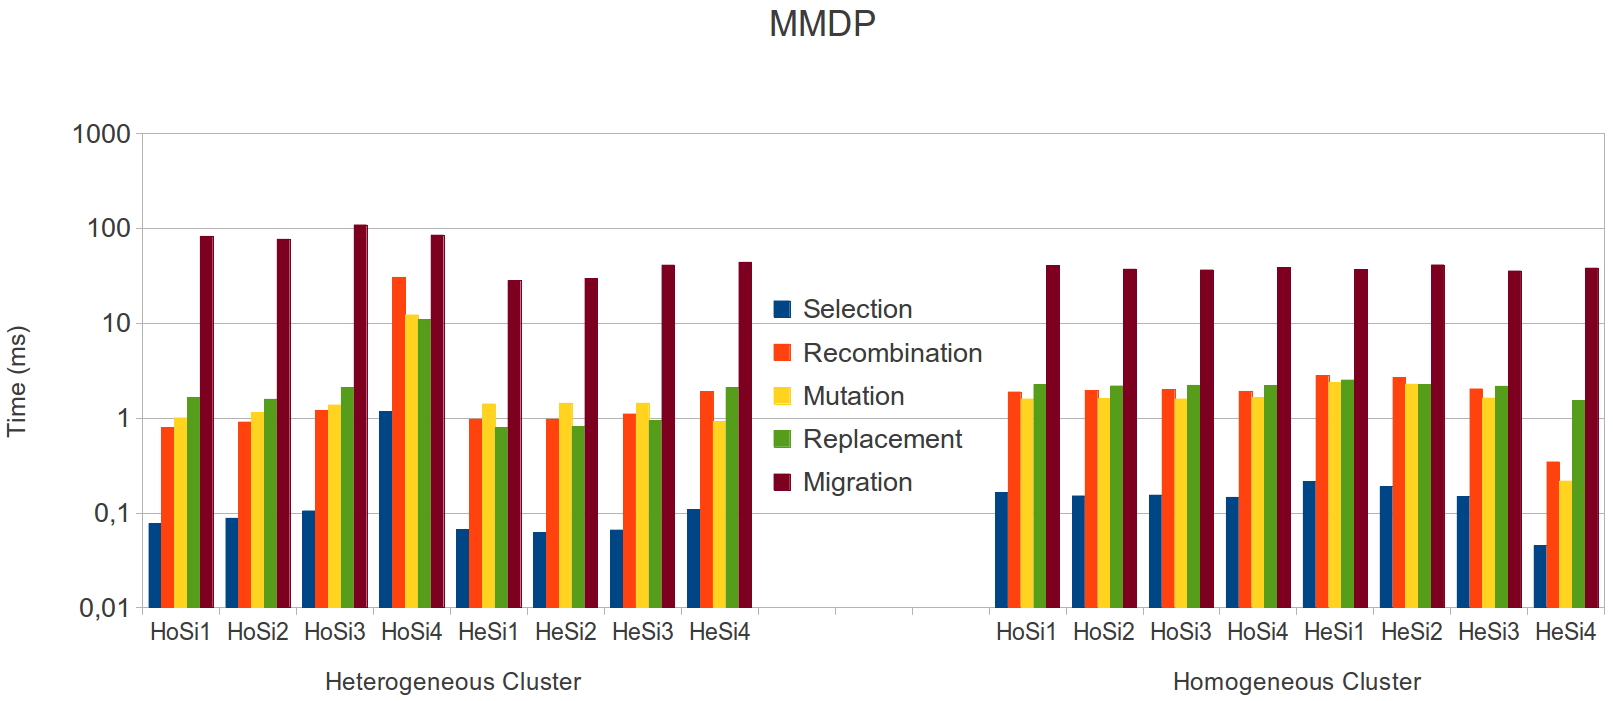
\includegraphics[scale =0.19] {gfx/adaptiveresults/timingMMDP.png}
\caption{Average running time in each stage of the algorithm for the MMDP problem.}
\label{fig:MMDPbars}
\end{SCfigure}

\begin{SCfigure}[htb]
\centering
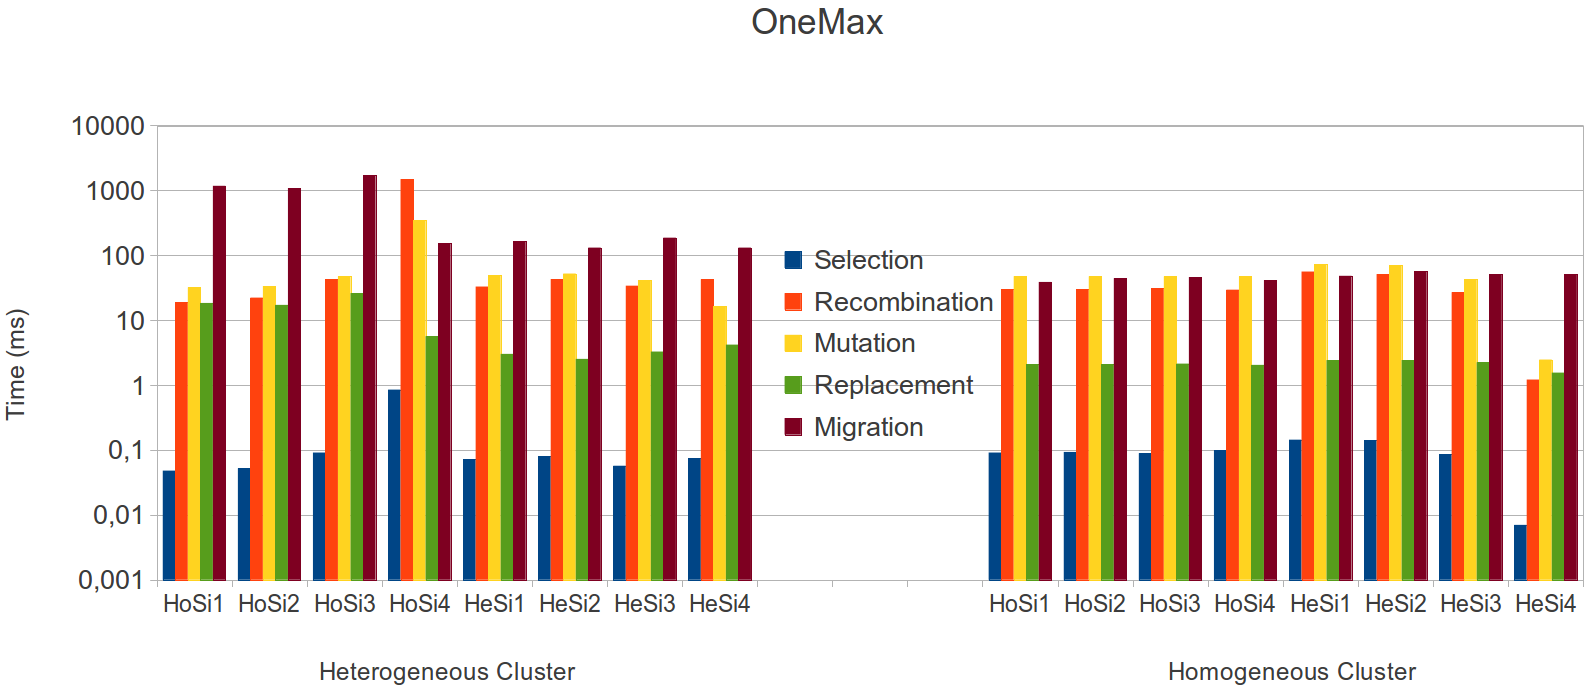
\includegraphics[scale =0.19] {gfx/adaptiveresults/timingONEMAX.png}
\caption{Average running time in each stage of the algorithm for the ONEMAX problem.}
\label{fig:ONEMAXbars}
\end{SCfigure}

\begin{SCtable}[][htb]
\resizebox{11cm}{!}{
\begin{tabular}{ccccccc}
\hline
\multicolumn{6}{>{\columncolor{colorCorporativoSuave}}c}{Heterogeneous Cluster} \\ \hline \hline
\rowcolor{colorCorporativoMasSuave}Node    & Selection     & Recombination     & Mutation      & Replacement       & Migration         \\ \hline
\rowcolor{colorCorporativoSuave}HoSi HeN1    & 0.077 $\pm$  0.170 &  0.788  $\pm$ 0.779  & 1.004  $\pm$ 0.187 &  1.648  $\pm$ 20.185 & 82.458  $\pm$ 143.266 \\ \hline
\rowcolor{colorCorporativoMasSuave}HoSi HeN2    & 0.088 $\pm$  0.190 &  0.907 $\pm$  0.932  & 1.145  $\pm$ 0.425 &  1.579  $\pm$ 17.907 & 76.725  $\pm$ 126.360\\ \hline
\rowcolor{colorCorporativoSuave}HoSi HeN3    & 0.105 $\pm$  0.163 &  1.207 $\pm$  0.927  & 1.374  $\pm$ 0.301 &  2.108  $\pm$ 21.848 & 108.605 $\pm$ 142.633\\ \hline
\rowcolor{colorCorporativoMasSuave}HoSi HeN4    & 1.165 $\pm$  1.526 &  30.445$\pm$  59.553 & 12.221 $\pm$ 7.412 &  10.978 $\pm$ 57.135 & 84.936  $\pm$ 0.000\\ \hline \hline
\rowcolor{colorCorporativoSuave}HeSi HeN1    & 0.067 $\pm$  0.065  & 0.973  $\pm$ 0.403 &  1.411 $\pm$  0.166 &  0.790  $\pm$ 6.266 &  28.081 $\pm$ 42.169 \\ \hline
\rowcolor{colorCorporativoMasSuave}HeSi HeN2    & 0.062 $\pm$  0.075  & 0.973  $\pm$ 0.470 &  1.433 $\pm$  0.265 &  0.811  $\pm$ 7.056 &  29.667 $\pm$ 48.702 \\ \hline
\rowcolor{colorCorporativoSuave}HeSi HeN3    & 0.066 $\pm$  0.108  & 1.104  $\pm$ 0.346 &  1.435 $\pm$  0.296 &  0.937  $\pm$ 7.072 &  40.964 $\pm$ 40.027 \\ \hline
\rowcolor{colorCorporativoMasSuave}HeSi HeN4    & 0.109 $\pm$  0.257  & 1.895  $\pm$ 5.611 &  0.913 $\pm$  0.834 &  2.085  $\pm$ 5.626 &  43.880 $\pm$ 7.535 \\ \hline 

\hline \hline
\multicolumn{6}{>{\columncolor{colorCorporativoSuave}}c}{Homogeneous Cluster} \\ \hline  \hline                               
\rowcolor{colorCorporativoMasSuave}Node    & Selection     & Recombination     & Mutation      & Replacement       & Migration \\ \hline
\rowcolor{colorCorporativoSuave}HoSi HoN1    & 0.163 $\pm$  0.223 &  1.884 $\pm$  2.386  & 1.591  $\pm$ 0.479 &  2.254  $\pm$ 5.513  & 40.256  $\pm$ 8.726\\ \hline
\rowcolor{colorCorporativoMasSuave}HoSi HoN2    & 0.151 $\pm$  0.212 &  1.952 $\pm$  2.876  & 1.597  $\pm$ 0.574 &  2.178  $\pm$ 4.922  & 37.110  $\pm$ 6.999\\ \hline
\rowcolor{colorCorporativoSuave}HoSi HoN3    & 0.154 $\pm$  0.206 &  1.990 $\pm$  3.010  & 1.591  $\pm$ 0.577 &  2.215  $\pm$ 4.743  & 36.413  $\pm$ 5.266\\ \hline
\rowcolor{colorCorporativoMasSuave}HoSi HoN4    & 0.146 $\pm$  0.196 &  1.913 $\pm$  2.697  & 1.651  $\pm$ 1.167 &  2.194  $\pm$ 5.124  & 38.429  $\pm$ 6.192\\ \hline \hline
\rowcolor{colorCorporativoSuave}HeSi HoN1    & 0.214 $\pm$  0.288  & 2.800  $\pm$ 3.793 &  2.359 $\pm$  0.691 &  2.516  $\pm$ 4.706 &  36.972 $\pm$ 4.214 \\ \hline
\rowcolor{colorCorporativoMasSuave}HeSi HoN2    & 0.190 $\pm$  0.252  & 2.672  $\pm$ 3.902 &  2.277 $\pm$  0.649 &  2.261  $\pm$ 4.546 &  41.171 $\pm$ 9.672 \\ \hline
\rowcolor{colorCorporativoSuave}HeSi HoN3    & 0.148 $\pm$  0.208  & 2.030  $\pm$ 3.161 &  1.623 $\pm$  0.500 &  2.164  $\pm$ 4.512 &  35.551 $\pm$  6.132 \\ \hline
\rowcolor{colorCorporativoMasSuave}HeSi HoN4    & 0.045 $\pm$  0.052  & 0.345  $\pm$ 1.121 &  0.217 $\pm$  0.142 &  1.531  $\pm$ 4.856 &  38.106 $\pm$ 9.251 \\ \hline
\end{tabular}
}
\caption{Times of the stages of the algorithm for the MMDP problem (in ms).}
\label{tab:mmdptimes}
\end{SCtable}








\begin{SCtable}[][htb]
\resizebox{11cm}{!}{
\begin{tabular}{ccccccc}
\hline
\multicolumn{6}{>{\columncolor{colorCorporativoSuave}}c}{Heterogeneous Cluster} \\ \hline \hline
\rowcolor{colorCorporativoMasSuave}Node    & Selection     & Recombination     & Mutation      & Replacement       & Migration         \\ \hline
\rowcolor{colorCorporativoSuave}HoSi HeN1  &  0.048 $\pm$  0.043  & 18.713 $\pm$ 13.454 & 31.984 $\pm$ 2.104  & 18.375 $\pm$ 197.676 & 1172.986  $\pm$  1108.388 \\ \hline
\rowcolor{colorCorporativoMasSuave}HoSi HeN2  &  0.052 $\pm$  0.051  & 22.266 $\pm$  22.716 & 33.553 $\pm$ 4.931 &  17.176 $\pm$ 180.580 & 1085.508  $\pm$  995.382 \\ \hline
\rowcolor{colorCorporativoSuave}HoSi HeN3  &  0.091 $\pm$  1.005  & 42.634 $\pm$ 21.621  & 47.674 $\pm$ 0.546 &  26.094 $\pm$ 252.667 & 1708.402 $\pm$   1207.925 \\ \hline
\rowcolor{colorCorporativoMasSuave}HoSi HeN4  &  0.851  $\pm$ 0.435  & 1491.568 $\pm$ 1185.723 & 344.872$\pm$ 6.634 &  5.655  $\pm$ 16.175 & 154.019 $\pm$0.000 \\ \hline \hline
\rowcolor{colorCorporativoSuave}HeSi HeN1 &   0.072 $\pm$  0.063 &  32.917 $\pm$ 26.792 & 49.103 $\pm$ 2.655  & 3.023 $\pm$  27.647 & 163.479 $\pm$157.172 \\ \hline
\rowcolor{colorCorporativoMasSuave}HeSi HeN2 &   0.080 $\pm$  0.092 &  43.001 $\pm$ 51.680 & 52.288 $\pm$ 13.210 & 2.527 $\pm$  21.861 & 131.063 $\pm$124.404 \\ \hline
\rowcolor{colorCorporativoSuave}HeSi HeN3 &   0.057 $\pm$  0.052 &  33.951 $\pm$ 15.063 & 41.375 $\pm$ 1.707  & 3.284 $\pm$  30.170 & 186.467 $\pm$163.906 \\ \hline
\rowcolor{colorCorporativoMasSuave}HeSi HeN4 &   0.075 $\pm$  0.107 &  42.443 $\pm$ 88.536 & 16.236 $\pm$ 12.028 & 4.194 $\pm$  33.119 & 131.135 $\pm$144.359 \\ \hline 

\hline \hline
\multicolumn{6}{>{\columncolor{colorCorporativoSuave}}c}{Homogeneous Cluster} \\ \hline  \hline                               
\rowcolor{colorCorporativoMasSuave}Node    & Selection     & Recombination     & Mutation      & Replacement       & Migration \\ \hline
\rowcolor{colorCorporativoSuave}HoSi HoN1  &  0.091 $\pm$  0.078  & 29.969 $\pm$ 21.459 & 47.445 $\pm$ 2.194 &  2.073 $\pm$  6.970 &  38.782 $\pm$ 40.369 \\ \hline
\rowcolor{colorCorporativoMasSuave}HoSi HoN2  &  0.093 $\pm$  0.082  & 30.119 $\pm$ 22.029 & 47.247 $\pm$ 2.146 &  2.108 $\pm$  7.440 &  44.303 $\pm$ 42.759 \\ \hline
\rowcolor{colorCorporativoSuave}HoSi HoN3  &  0.089 $\pm$  0.080  & 30.951 $\pm$ 21.904 & 47.103 $\pm$ 2.031 &  2.138 $\pm$  8.006 &  46.107 $\pm$ 47.351 \\ \hline
\rowcolor{colorCorporativoMasSuave}HoSi HoN4  &  0.098 $\pm$  0.075  & 29.468 $\pm$ 20.876 & 47.086 $\pm$ 1.856 &  2.043 $\pm$  7.491 &  41.458 $\pm$ 44.970 \\ \hline \hline
\rowcolor{colorCorporativoSuave}HeSi HoN1 &   0.144 $\pm$  0.151 &  56.124 $\pm$ 48.229 & 72.811 $\pm$ 5.177  & 2.424 $\pm$  9.056  & 48.165  $\pm$57.798 \\ \hline
\rowcolor{colorCorporativoMasSuave}HeSi HoN2 &   0.141 $\pm$  0.152 &  51.226 $\pm$ 41.016 & 70.047 $\pm$ 4.152  & 2.427 $\pm$  10.890 & 57.152  $\pm$74.177 \\ \hline
\rowcolor{colorCorporativoSuave}HeSi HoN3 &   0.086 $\pm$  0.088 &  26.932 $\pm$ 20.460 & 42.963 $\pm$ 3.935  & 2.239 $\pm$  8.658  & 51.014  $\pm$49.648 \\ \hline
\rowcolor{colorCorporativoMasSuave}HeSi HoN4 &   0.007 $\pm$  0.008 &  1.215  $\pm$ 1.133  & 2.470  $\pm$ 0.098  & 1.553 $\pm$  10.078 & 50.498 $\pm$ 63.983 \\ \hline
\end{tabular}
}
\caption{Times of the stages of the algorithm for the OneMax problem (in ms).}
\label{tab:onemaxtimes}
\end{SCtable}